\documentclass[border=10px]{standalone}
\usepackage{tikz}
\usetikzlibrary{patterns}
\usetikzlibrary{shapes.arrows}
\usepackage{amssymb}
\usetikzlibrary{calc}
\usetikzlibrary{positioning}
\usepackage{verbatim}
\begin{document}
	
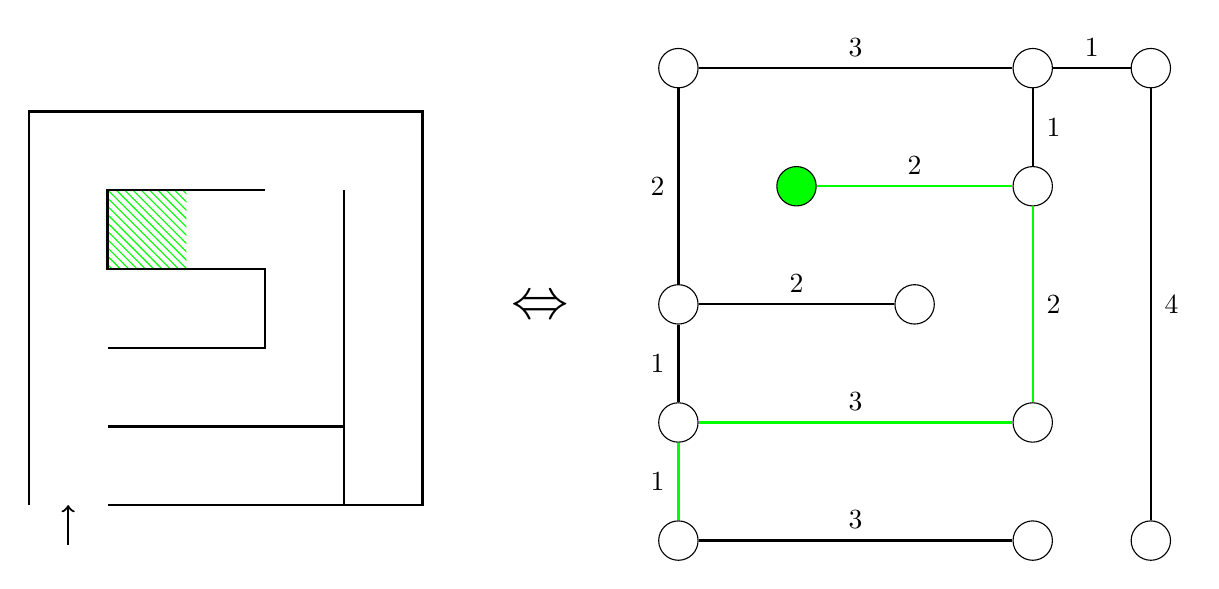
\begin{tikzpicture}[scale=1]
		
		\draw[thick, ,draw=none, pattern=north west lines, pattern color=green] (1,3) rectangle (2,4);
		\draw[thick] (0,0) -- (0,5) -- (5,5) -- (5,0) -- (1,0);
		\draw[thick] (4,0) -- (4,4);
		\draw[thick] (4,1) -- (1,1);
		\draw[thick] (1,2) -- (3,2) -- (3,3) -- (1,3) -- (1,4) -- (3,4);
		
		\draw[thick, ->] (.5,-.5) -- (.5,0);
		
		\node[] at (6.5,2.5) {\huge $\Leftrightarrow$};
		
		\tikzset{every node/.style={minimum size=.5cm, align=center,anchor=center, on grid,x=1.5cm,y=1.5cm}}
		\node[draw=black, circle] 							(A) at (5.5,-.3) {};
		\node[above=1 of A, draw=black, circle] 				(B) {};
		\node[above=1 of B, draw=black, circle] 				(C) {};
		\node[above=2 of C, draw=black, circle] 				(D) {};
		\node[right=3 of D, draw=black, circle] 				(E) {};
		\node[right=1 of E, draw=black, circle] 				(F) {};
		\node[below=4 of F, draw=black, circle] 				(G) {};
		\node[below=1 of E, draw=black, circle] 				(H) {};
		\node[left=2 of H, draw=black,fill=green, circle] 	(I) {};
		\node[below=2 of H, draw=black, circle] 				(J) {};
		\node[right=2 of C, draw=black, circle] 				(K) {};
		\node[right=3 of A, draw=black, circle] 				(L) {};
		
		\draw[thick,draw=green] (A) -- node[left] 	{1} (B) ;
		\draw[thick] 			(B) -- node[left] 	{1} (C);
		\draw[thick] 			(C) -- node[left] 	{2} (D);
		\draw[thick] 			(D) -- node[above] 	{3} (E);
		\draw[thick] 			(E) -- node[above] 	{1} (F);
		\draw[thick] 			(F) -- node[right] 	{4} (G);
		\draw[thick] 			(E) -- node[right] 	{1} (H);
		\draw[thick,draw=green] (H) -- node[above] 	{2} (I);
		\draw[thick,draw=green] (H) -- node[right] 	{2} (J);
		\draw[thick,draw=green] (J) -- node[above] 	{3} (B);
		\draw[thick] 			(A) -- node[above] 	{3} (L);
		\draw[thick] 			(C) -- node[above] 	{2} (K);
		
	\end{tikzpicture}
\end{document}